\section{太阳能电池的原理及结构}

目前,市售的太阳能电池以晶体硅太阳能电池为主。本节以晶体硅太阳能电池为例,
对太阳能电池的原理和结构进行介绍。

\subsection{太阳能电池的原理}

在抽象的意义下,晶体硅太阳能电池就是一个大的 p-n 结。当外界的光子流照射
晶体硅时,若光子的能量 $E = h\nu$ 不小于晶体硅的禁带宽度,则满带的电子就会
吸收该光子,并被激发到空带中。根据 Bloch 理论,空带中被激发出的少量电子可
以被视为自由电子,而满带中缺失的少量电子可以被视为带有正电荷的“空穴”。
对于普通的晶体硅,产生的电子-空穴对会以一定速率重新复合(即,被激发的电子
重新跃迁回满带,并辐射光子),电子-空穴对的产生率与复合率相等,没有宏观
电流。然而,由于 p-n 结耗尽区中存在极强的电场,在耗尽区中产生的电子和空穴
会在电场作用下向相反方向漂移,从而形成宏观的光电流。设 p-n 结的截面积是
$A$,耗尽区的宽度是 $W$,则光电流正比于单位时间内到达耗尽区内部的光子数:
\begin{equation} \label{eqn:LightCurrent}
I_L = K \cdot q_e L(W \cdot A)
\end{equation}
这里 $L$ 是光通量,$q_e$ 是电子的电荷量,$K$ 是和光的频率、半导体内部能带
结构等有关的常数。由于耗尽区很薄,$W$ 趋于 $0$ ,这里并不需要使用
Lambert-Beer 形式的吸收定律。

在太阳能电池不短路的情况下,光电流通过负载,将产生电压降 $V$。由于太阳能
电池本身是一个 p-n 结,在 $V$ 的偏置下,将产生电流:
\begin{equation} \label{eqn:Shockley}
I_F = I_S \left[ exp \left(\frac{q_e V}{k_B T} \right) - 1 \right]
\end{equation}
这就是Shockley 二极管方程,电流 $I_F$ 通常称为光电池的
暗电流。暗电流的方向与光电流 $I_L$ 相反,故总电流为:
\begin{equation} \label{eqn:TotalCurrent}
I = I_F - I_L
\end{equation}
短路时没有暗电流,故短路电流的大小和光电流相同:
\begin{equation} \label{eqn:SCCurrent}
I_{SC} = -I_L
\end{equation}

\subsection{晶体硅太阳能电池的内部结构}

晶体硅太阳能电池的 p-n 结是在厚度为 $200\mu m \sim 500\mu m$ 的 p 型硅晶体
上制作一 $0.2 \mu m \sim 0.5 \mu m$ 深的 n 型半导体层而成。 $n$ 层表面为
感光面,感光面用碱腐蚀成绒面,并喷涂一层减反射膜,以减小表面反射,提高
光电转化效率。

减反射膜下方印制主电极(busbar)和栅电极(finger),
主电极宽度约 $2mm$ ,栅电极宽度为
$0.1mm$,间距为 $3mm$ 。主电极和栅电极组成太阳能电池的负极。在这种设计
下,负极的总面积较小,减小了感光面积的损失。同时, $n$ 区的各个位置距离
栅电极都较近,有利于收集载流子,减少了载流子的复合损失。

在 p 衬底的下表面印制一层金属,作为正极,称为背电极。正负极和硅晶体之间
都形成良好的欧姆接触。整个太阳能电池的结构如图 \ref{fig:semantics} 所示。

\begin{figure}
\centering
\includegraphics[width=.8\textwidth]{Figure/semantics.pdf}
\caption{太阳能电池结构示意图}
\label{fig:semantics}
\end{figure}

\subsection{晶体硅太阳能电池的常见缺陷}

晶体硅太阳能电池中,任何组件的故障都可导致缺陷。下面简要介绍各种缺陷的成
因和形态。

固有缺陷是生产太阳能电池所用的硅材料本身的缺陷。理想状态下,
单晶硅是具有金刚石型晶胞的晶体,但这在现实中不可能。在加工过程中,杂质原子
会混入硅材料,同时由于温度、应力的不均,硅材料中将产生位错、层错、晶格空
位、间隙缺陷、 Frenkel 缺陷、 Schottky 缺陷等晶格缺陷。晶体缺陷将在很大
程度上影响局部的能带结构(甚至形成新的能级),可能提高载流子的复合率,导
致光子激发的电子-空穴对不能到达电极,从而形成低光电转化效率区域。

外部缺陷是在制造太阳能电池板的工艺过程中产生的,例如夹具和
量具在接触硅晶体时都可能导致表面污染,栅电极在印制过程中可能出现断线,
加工过程中电池板受到冲击可能出现裂纹,减反射膜可能过厚或过薄(均会影响
频率响应)。

图 \ref{fig:PLimage} 是采用 PL 法获得的一组缺陷图像,其中 a 是 \ch{Si3N4}
减反射膜上一处半椭圆形的缺损, b 是激光切割系统故障导致样品边缘出现的微
裂纹, c 是用螺旋测微计测量样品厚度时造成的表面污染, d 是硅片炉内退火时
温度不均产生的固有缺陷, e 是使用 RCA 标准清洗法处理硅片时夹具留下的痕迹,
f 是被严重污染的硅片\cite{FastPL}。

\begin{figure}
\centering
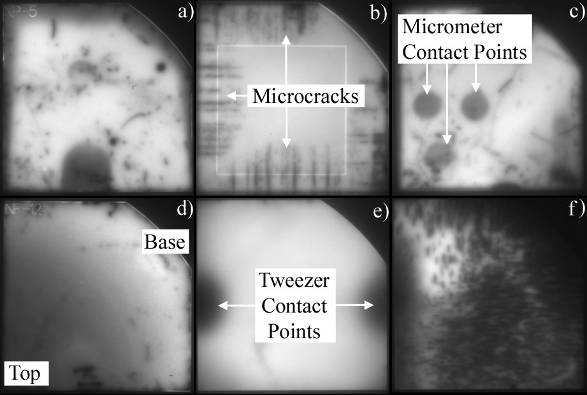
\includegraphics[width=.6\textwidth]{Figure/PLimage.png}
\caption{一些太阳能电池缺陷的 PL 图像}
\label{fig:PLimage}
\end{figure}
